\documentclass[00-GLMregslides.tex]{subfiles}
\begin{document}

%================================================================================================%
%\begin{frame}[fragile]
%	
%	\frametitle{Ordinal Logistic Regression with \texttt{R}}
%	\Large
%	The code below contains two commands (the first command falls on multiple lines) and is used to create this graph to test the proportional odds assumption. Basically, we will graph predicted logits from individual logistic regressions with a single predictor where the outcome groups are defined by either apply $>=$ 2 and apply $>=$ 3. 
%	
%\end{frame}

\begin{frame}
\begin{center}
	
\end{center}	\begin{figure}
\centering
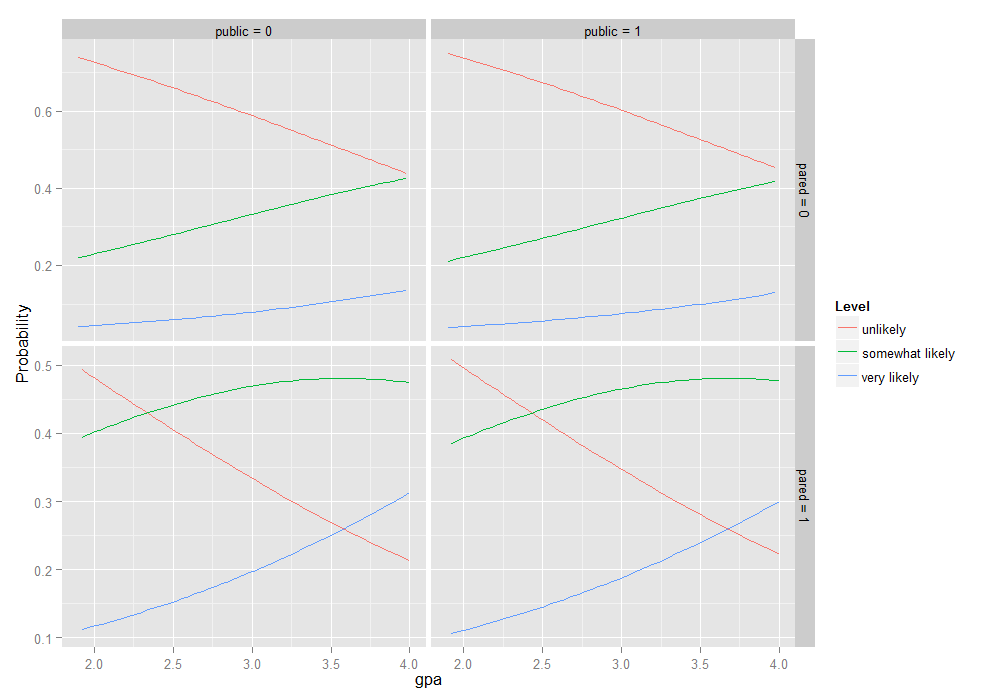
\includegraphics[width=0.7\linewidth]{ologit2}
\caption{}
\label{fig:ologit2}
\end{figure}

\end{frame}
%%================================================================================================%
%\begin{frame}[fragile]
%	
%	\frametitle{Ordinal Logistic Regression with \texttt{R}}
%	\Large
%	
%	If the difference between predicted logits for varying levels of a predictor, say pared, are the same whether the outcome is defined by apply $>=$ 2 or apply $>=$3, then we can be confident that the proportional odds assumption holds. In other words, if the difference between logits for pared = 0 and pared = 1 is the same when the outcome is apply $>=$ 2 as the difference when the outcome is apply $>=$ 3, then the proportional odds assumption likely holds.
%	
%\end{frame}
%%================================================================================================%
%\begin{frame}[fragile]
%	
%	\frametitle{Ordinal Logistic Regression with \texttt{R}}
%	\Large
%	The first command creates the function that estimates the values that will be graphed. The first line of this command tells R that sf is a function, and that this function takes one argument, which we label y. The sf function will calculate the log odds of being greater than or equal to each value of the target variable. For our purposes, we would like the log odds of apply being greater than or equal to 2, and then greater than or equal to 3. 
%	
%\end{frame}
%%================================================================================================%
%\begin{frame}[fragile]
%	
%	\frametitle{Ordinal Logistic Regression with \texttt{R}}
%	\Large
%	
%	Depending on the number of categories in your dependent variable, and the coding of your variables, you may have to edit this function. Below the function is configured for a y variable with three levels, 1, 2, 3. If your dependent variable has 4 levels, labeled 1, 2, 3, 4 you would need to add 'Y$>=$4'=qlogis(mean(y $>=$ 4)) (minus the quotation marks) inside the first set of parentheses. If your dependent variable were coded 0, 1, 2 instead of 1, 2, 3, you would need to edit the code, replacing each instance of 1 with 0, 2 with 1, and so on. Inside the sf function we find the qlogis function, which transforms a probability to a logit. 
%	
%\end{frame}
%%================================================================================================%
%\begin{frame}[fragile]
%	
%	\frametitle{Ordinal Logistic Regression with \texttt{R}}
%	\Large
%	So, we will basically feed probabilities of apply being greater than 2 or 3 to qlogis, and it will return the logit transformations of these probabilites. Inside the qlogis function we see that we want the log odds of the mean of y $>=$ 2. When we supply a y argument, such as apply, to function sf, y $>=$ 2 will evaluate to a 0/1 (FALSE/TRUE) vector, and taking the mean of that vector will give you the proportion of or probability that apply $>=$ 2.
%\end{frame}
%%================================================================================================%
%\begin{frame}[fragile]
%	
%	\frametitle{Ordinal Logistic Regression with \texttt{R}}
%	\Large
%	\begin{itemize}
%	\item The second command below calls the function sf on several subsets of the data defined by the predictors. 
%	\item In this statement we see the summary function with a formula supplied as the first argument. 
%	\item When R sees a call to summary with a formula argument, it will calculate descriptive statistics for the variable on the left side of the formula by groups on the right side of the formula and will return the results in a nice table. 
%	\end{itemize}
%\end{frame}
%%================================================================================================%
%\begin{frame}[fragile]
%	
%	\frametitle{Ordinal Logistic Regression with \texttt{R}}
%	\Large
%	
%	By default, summary will calculate the mean of the left side variable. So, if we had used the code summary(as.numeric(apply) ~ pared + public + gpa) without the fun argument, we would get means on apply by pared, then by public, and finally by gpa broken up into 4 equal groups. However, we can override calculation of the mean by supplying our own function, namely sf to the fun= argument. The final command asks R to return the contents to the object s, which is a table.
%\end{frame}
%================================================================================================%
\end{document}